% Secure Energy-Efficient Scheduling for AI Workloads — A0 portrait research poster
% Layout reproduces the SciFig "A0 Portrait — Classic" template specification (Navy):
%   3 columns in a 1.2 : 1.6 : 1.2 ratio, title 85 pt, authors 56 pt, section headings 45 pt,
%   body 26 pt, captions/references 24 pt, Navy #1B365D on white, body text #1A1A1A, Arial-metric font.
% Build:  cd poster && lualatex poster.tex   (two passes; requires `seas report` to have written generated/results.tex)
\documentclass{article}
\usepackage[paperwidth=841mm,paperheight=1189mm,margin=0mm]{geometry}
\usepackage{fontspec}
\usepackage{unicode-math}
\setmainfont{Liberation Sans}
\setsansfont{Liberation Sans}
\setmathfont{DejaVu Math TeX Gyre}
\usepackage{xcolor}
\usepackage{graphicx}
\graphicspath{{../figures/}{figures/}}
\usepackage{tikz}
\usetikzlibrary{arrows.meta,positioning,calc,fit,backgrounds}
\usepackage{enumitem}
\usepackage{qrcode}
\usepackage{microtype}
\usepackage[hidelinks]{hyperref}
\pagestyle{empty}
\setlength{\parindent}{0pt}

\definecolor{navy}{HTML}{1B365D}
\definecolor{ink}{HTML}{1A1A1A}
\definecolor{muted}{HTML}{5A5A5A}
\definecolor{seas}{HTML}{009E73}
\definecolor{eftc}{HTML}{0072B2}
\definecolor{warn}{HTML}{C0392B}
\definecolor{tint}{HTML}{EEF2F7}
\definecolor{tintgreen}{HTML}{E6F5EF}
\definecolor{tintred}{HTML}{FBECEA}

% generated by `seas report` from results/ — do not edit
\newcommand{\HOneEnergyRel}{−0.6}
\newcommand{\HOneEnergyLo}{−1.1}
\newcommand{\HOneEnergyHi}{−0.1}
\newcommand{\HOnePEnergy}{0.020}
\newcommand{\HOneMissSeas}{3.7}
\newcommand{\HOneMissEft}{7.8}
\newcommand{\HOneNIUpper}{−3.2}
\newcommand{\HOneNIMargin}{2}
\newcommand{\HOnePNI}{< 0.001}
\newcommand{\HOneVerdict}{supported}
\newcommand{\HOnePHolm}{0.040}
\newcommand{\AblSeasVsSlack}{−1.6}
\newcommand{\AblSlackVsEft}{1.0}
\newcommand{\HTwoSlope}{−1.6}
\newcommand{\HTwoSlopeLo}{−2.4}
\newcommand{\HTwoSlopeHi}{−0.8}
\newcommand{\HTwoPHolm}{1.000}
\newcommand{\HTwoPTwoSided}{< 0.001}
\newcommand{\HTwoVerdict}{not supported}
\newcommand{\HTwoGainZero}{1.4}
\newcommand{\HTwoGainMax}{0.2}
\newcommand{\HThreeEnergyRel}{−1.0}
\newcommand{\HThreeMissVsGreedy}{−10.3}
\newcommand{\HThreePHolm}{0.002}
\newcommand{\HThreeVerdict}{supported}
\newcommand{\HFourDiff}{11.5}
\newcommand{\HFourVerdict}{binding}
\newcommand{\GreedyEnergyRel}{−4.8}
\newcommand{\FifoEnergyKJ}{2147}
\newcommand{\EftEnergyKJ}{377}
\newcommand{\SeasEnergyKJ}{375}
\newcommand{\IdleWindowKJ}{360}
\newcommand{\NoChoice}{10}
\newcommand{\Violations}{0}
\newcommand{\DynShare}{51}
\newcommand{\TotWindowRel}{−0.28}
\newcommand{\TotWindowLo}{−0.53}
\newcommand{\TotWindowHi}{−0.00}
\newcommand{\TotGatedRel}{+0.17}
\newcommand{\TotGatedLo}{−0.24}
\newcommand{\TotGatedHi}{+0.62}
\newcommand{\PerWorkRel}{−3.6}
\newcommand{\PerWorkLo}{−4.1}
\newcommand{\PerWorkHi}{−3.2}
\newcommand{\WorkRel}{+3.2}
\newcommand{\WorkLo}{+2.3}
\newcommand{\WorkHi}{+4.1}
\newcommand{\GapSeas}{0.4}
\newcommand{\GapEft}{2.4}
\newcommand{\GapGreedy}{0.0}
\newcommand{\SeasWinsSeeds}{20}
\newcommand{\NSeeds}{30}
\newcommand{\IdleEmptyShare}{36}
\newcommand{\HeadroomShare}{0.2}
\newcommand{\HeadroomMax}{0.7}
\newcommand{\SlackMiss}{3.7}
\newcommand{\AlphaSameSeeds}{27}
\newcommand{\AlphaNSeeds}{30}
\newcommand{\AlphaMaxDiff}{0.00}
\newcommand{\AlphaZeroIsSlack}{yes}
\newcommand{\NRuns}{4\,380}

\newcommand{\seasname}{\leavevmode{\bfseries\color{seas}seas}}

% ---------- type scale (SciFig) ----------
\newcommand{\bodysize}{\fontsize{26}{33}\selectfont}
\newcommand{\capsize}{\fontsize{24}{29}\selectfont}
\newcommand{\refsize}{\fontsize{22.5}{27}\selectfont}
\newcommand{\headsize}{\fontsize{45}{52}\selectfont}

\renewcommand{\section}[1]{%
  \par\vspace{14mm}{\headsize\bfseries\color{navy}#1\par}\vspace{3mm}%
  {\color{navy}\rule{\linewidth}{1.6mm}}\par\vspace{7mm}}
\newcommand{\firstsection}[1]{%
  {\headsize\bfseries\color{navy}#1\par}\vspace{3mm}%
  {\color{navy}\rule{\linewidth}{1.6mm}}\par\vspace{7mm}}
\providecommand{\caption}{}\renewcommand{\caption}[1]{\par\vspace{3mm}{\capsize\color{muted}#1\par}}
\newcommand{\figfile}[2][]{\begin{center}\includegraphics[#1]{#2.pdf}\end{center}}

\setlist[itemize]{leftmargin=9mm,labelsep=4mm,itemsep=3mm,topsep=3mm,parsep=0mm,label={\color{navy}\rule[2.5mm]{3.2mm}{3.2mm}}}

\newcommand{\pill}[2]{{\setlength{\fboxsep}{2mm}\colorbox{#1}{\color{white}\bfseries\strut\,#2\,}}}
\newcommand{\verdictbox}[3]{% color, label, text
  \begin{tikzpicture}
    \node[draw=#1,line width=1.4mm,fill=white,rounded corners=4mm,inner sep=7mm,text width=\linewidth-16mm,align=left]
      {{\bfseries\color{#1}#2}\\[2mm]#3};
  \end{tikzpicture}}

% column geometry: 841 - 2*30 margins - 2*20 gutters = 741 mm; ratio 1.2 : 1.6 : 1.2
\newlength{\colA}\setlength{\colA}{222.3mm}
\newlength{\colB}\setlength{\colB}{296.4mm}
\newlength{\gut}\setlength{\gut}{20mm}

\newsavebox{\boxA}\newsavebox{\boxB}\newsavebox{\boxC}
\newlength{\toppos}\setlength{\toppos}{224mm}
\begin{document}
\color{ink}\bodysize

% ===================== HEADER BAND =====================
\begin{tikzpicture}[remember picture,overlay]
  \fill[navy] (current page.north west) rectangle ([yshift=-202mm]current page.north east);
  \node[anchor=north west,text width=640mm,align=left,inner sep=0] at ([xshift=30mm,yshift=-26mm]current page.north west)
    {\color{white}\fontsize{85}{94}\selectfont\bfseries\spaceskip=0.42em\relax Secure Energy-Efficient Scheduling\\for AI Workloads};
  \node[anchor=north west,text width=650mm,align=left,inner sep=0] at ([xshift=30mm,yshift=-114mm]current page.north west)
    {\color{white}\fontsize{36}{44}\selectfont Security-eligible, energy-aware placement of AI jobs on heterogeneous CPU/GPU clusters:\\a first reproducible prototype and a research programme};
  \node[anchor=north west,text width=650mm,align=left,inner sep=0] at ([xshift=30mm,yshift=-158mm]current page.north west)
    {\color{white}\fontsize{40}{48}\selectfont\bfseries Costin-Alexandru Deonise\quad{\mdseries\color{white!80!navy}·\quad Supervisor: Prof.\ Dr.\ Eng.\ Florin Pop}};
  \node[anchor=north west,text width=720mm,align=left,inner sep=0] at ([xshift=30mm,yshift=-179mm]current page.north west)
    {\color{white!85!navy}\fontsize{26}{32}\selectfont Faculty of Automatic Control and Computers, National University of Science and Technology POLITEHNICA Bucharest \,·\, PRECIS Research Centre};
  % QR in header (vector)
  \node[anchor=north east,fill=white,inner sep=4mm,rounded corners=2mm] (qr) at ([xshift=-30mm,yshift=-26mm]current page.north east)
    {\qrcode[height=100mm,level=M]{https://github.com/Maxxtra/phd}};
  \node[anchor=north,text width=120mm,align=center,inner sep=0] at ([yshift=-5mm]qr.south)
    {\color{white}\fontsize{24}{28}\selectfont github.com/Maxxtra/phd};
\end{tikzpicture}

% ===================== COLUMN 1 =====================
\begin{lrbox}{\boxA}\begin{minipage}[t]{\colA}\vspace{0pt}
\firstsection{Motivation}
Schedulers decide where every AI job runs, yet rarely ask what a placement costs in energy, and check whether a node may \emph{see the data} outside that decision.
\begin{itemize}
  \item AI's energy, carbon, water and land footprints are measurable and under-reported [7,\,8,\,9]; deployed inference is a major share [7].
  \item Confidential GPUs exist, but protected execution costs throughput (3–7\,\% for LLM inference on H100) [6]: secure nodes are slower and scarcer.
  \item Energy-aware schedulers [1–3] and intra-job energy tools [4] assume every node may run every job.
\end{itemize}

\section{Research question}
With security eligibility as a hard constraint, how much \emph{modelled} energy can placement on heterogeneous CPU/GPU clusters recover without missing more deadlines — and does security help or hurt?

\vspace{5mm}
{\capsize
\begin{tabular}{@{}p{14mm}p{\dimexpr\colA-16mm}@{}}
\textbf{\color{navy}H1} & \seasname{} uses less dynamic energy than EFT \emph{and} is non-inferior on misses (margin 2\,pp).\\[2mm]
\textbf{\color{navy}H2} & The gain grows with the share of security-constrained jobs.\\[2mm]
\textbf{\color{navy}H3} & Both hold under ±25\,\% execution-time estimation error.\\
\end{tabular}\par}
\vspace{3mm}
{\capsize\color{muted}Preregistered (configs hashed before any run); 30 paired seeds; Holm; non-inferiority by one-sided paired $t$-test.\par}

\section{Formal model}
Job $j$: work $w_j$, memory $m_j$, release $r_j$, deadline $d_j$, required capabilities $R_j$, energy weight $\alpha_j$. Node $n$: slots, memory $M_n$, capabilities $C_n$, throughput $\theta_{n,\tau}$, powers $P^{\mathrm{idle}}_n,P^{\mathrm{load}}_{n,\tau}$, protected slowdown $\sigma_n$.
\begin{center}
$\displaystyle S_{jn}=\mathbb{1}\!\left[R_j\subseteq C_n,\ m_j\le M_n\right]$\\[2mm]
$\displaystyle E_{jn}=\bigl(P^{\mathrm{load}}_{n,\tau_j}-P^{\mathrm{idle}}_n\bigr)\,\rho_{jn}\,\frac{w_j}{\theta_{n,\tau_j}}$\\[2mm]
$\displaystyle n^{*}=\operatorname*{arg\,min}_{\substack{n:\,S_{jn}=1\\ \mathrm{est}_{jn}+T_{jn}\le d_j}} \alpha_j\,\hat E_{jn}+(1-\alpha_j)\,\hat R_{jn}$
\end{center}
$\hat E,\hat R$: energy and predicted response time, normalised by the job's best option. Online, non-preemptive, least-slack-first; jobs that can no longer meet their deadline expire (same rule for all policies). Greedy heuristic; no optimality claim.

\section{Why a node is chosen}
\figfile{figC_decision_example}
\caption{A real decision record (S1, seed 0): the non-TEE GPU is fastest but ineligible; CPU confidential VMs would miss the deadline; the confidential GPU is chosen.}

\section{Limitations}
{\capsize
\begin{itemize}
  \item \textbf{Simulation only}: energies are modelled from synthetic profiles; no contention between co-located jobs; independent, non-preemptive jobs; one cluster.
  \item \textbf{Simulated security}: capability eligibility only; no enclave, encryption or attestation runs [5].
\end{itemize}\par}
\end{minipage}\end{lrbox}%
% ===================== COLUMN 2 =====================
\begin{lrbox}{\boxB}\begin{minipage}[t]{\colB}\vspace{0pt}
\firstsection{System and prototype}
\begin{center}
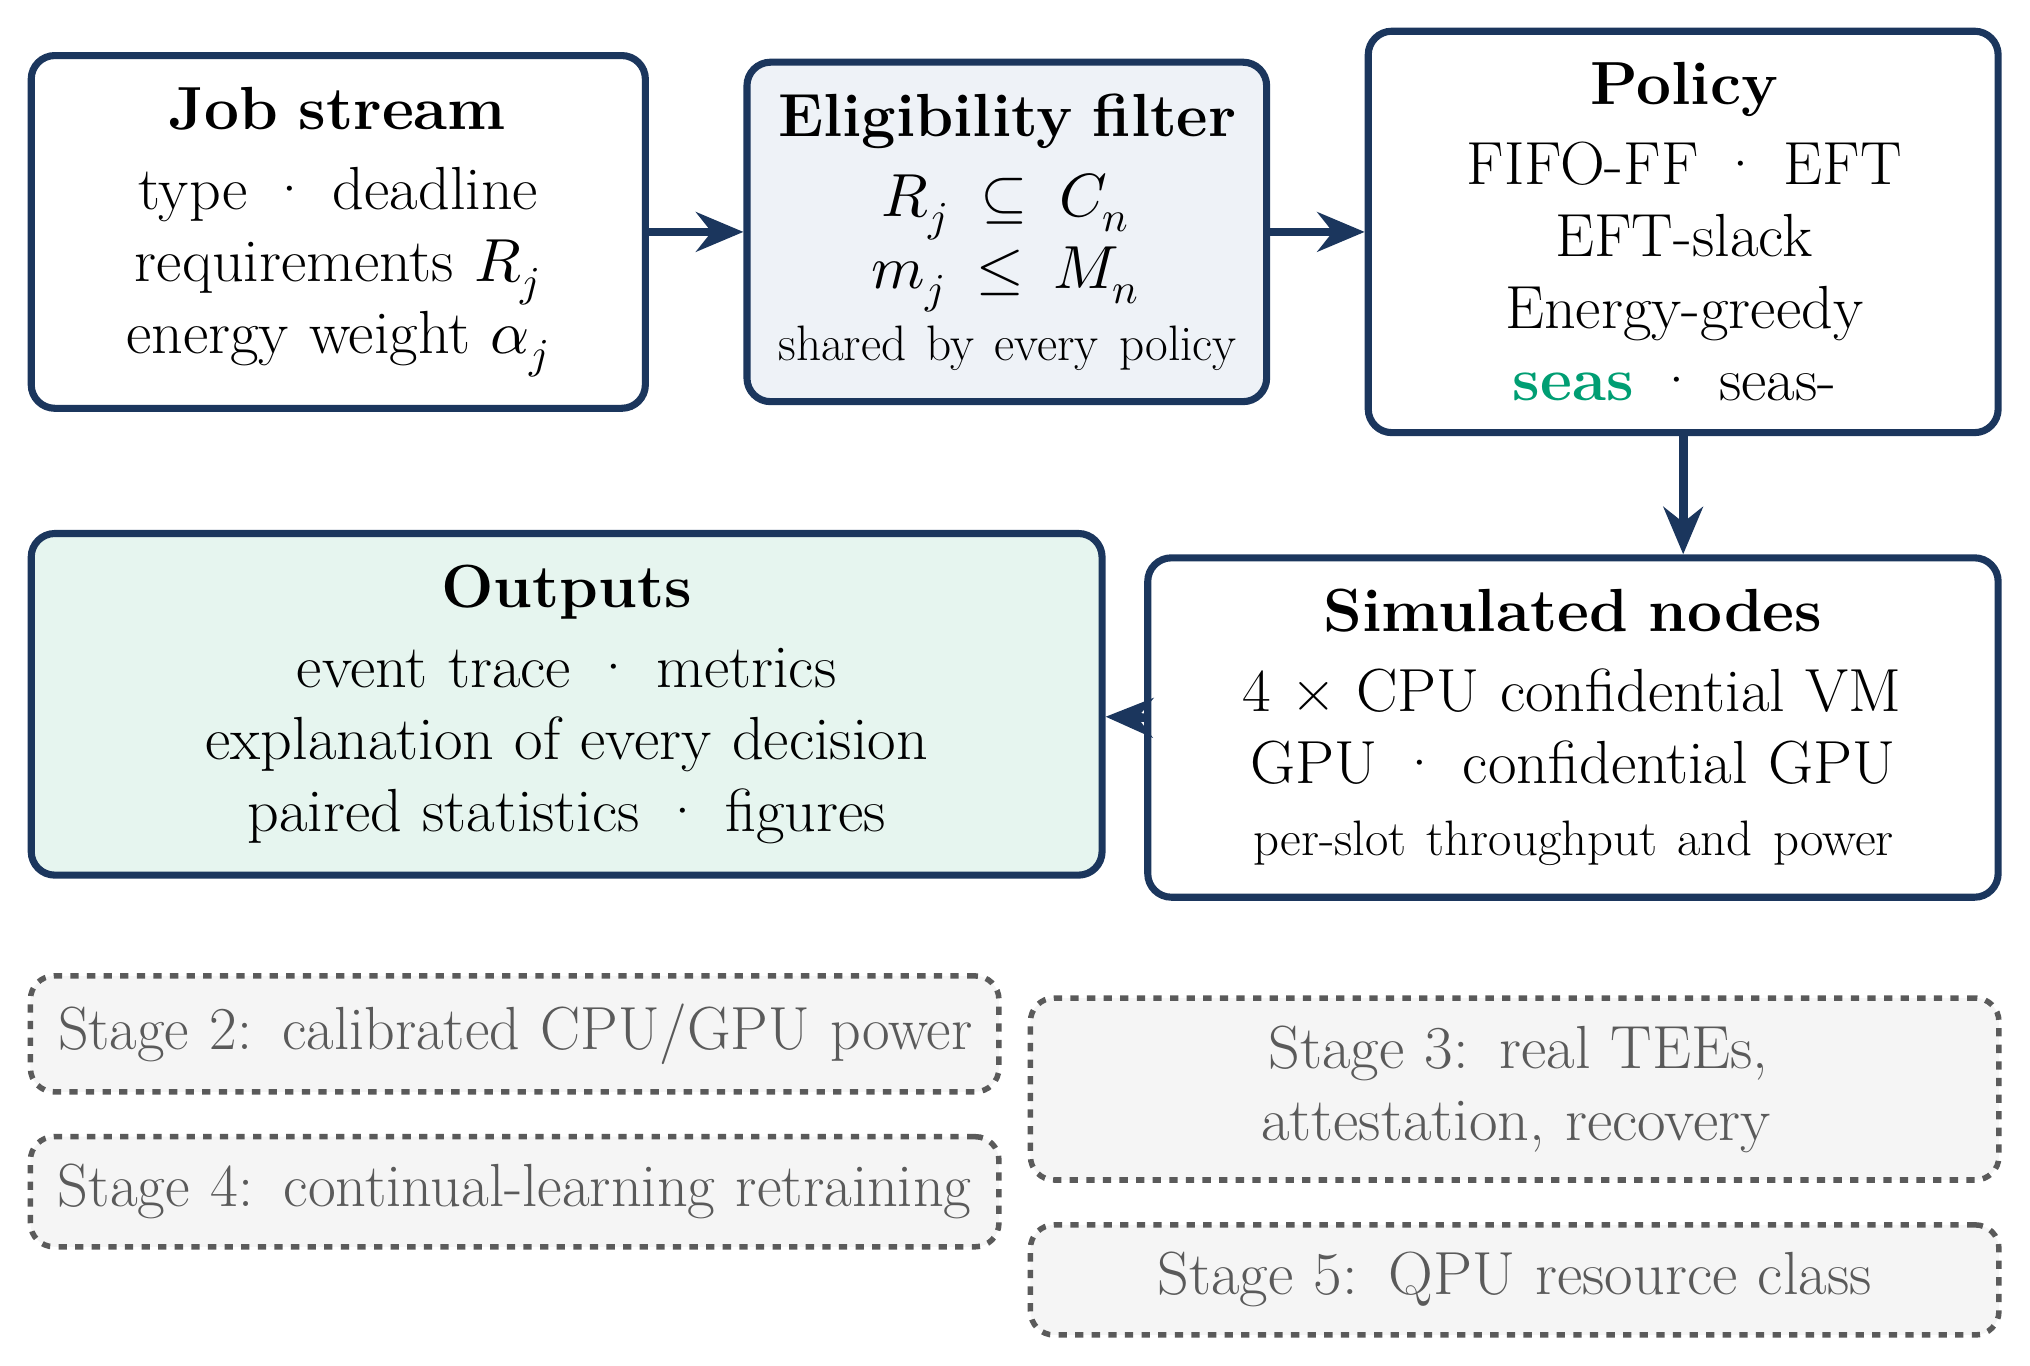
\begin{tikzpicture}[
    font=\fontsize{22}{26}\selectfont,
    box/.style={draw=navy,line width=0.9mm,rounded corners=3mm,align=center,inner sep=4mm,fill=white},
    impl/.style={box},
    plan/.style={draw=muted,line width=0.7mm,dashed,rounded corners=3mm,align=center,inner sep=3.5mm,fill=black!4,text=muted},
    arr/.style={-{Stealth[length=6mm,width=5mm]},line width=1.1mm,draw=navy}]
  \hyphenpenalty=10000
  \node[impl,text width=70mm] (jobs) {\textbf{Job stream}\\[1mm]type · deadline\\requirements $R_j$\\energy weight $\alpha_j$};
  \node[impl,text width=58mm,right=12mm of jobs,fill=tint] (filt) {\textbf{Eligibility filter}\\[1mm]$R_j\subseteq C_n$\\$m_j\le M_n$\\{\fontsize{18}{21}\selectfont shared by every policy}};
  \node[impl,text width=72mm,right=12mm of filt] (pol) {\textbf{Policy}\\[1mm]FIFO-FF · EFT\\EFT-slack\\Energy-greedy\\\textbf{\color{seas}seas} · seas-ε};
  \node[impl,text width=100mm,below=15mm of pol.south east,anchor=north east] (nodes) {\textbf{Simulated nodes}\\[1mm]4 × CPU confidential VM\\GPU · confidential GPU\\{\fontsize{18}{21}\selectfont per-slot throughput and power}};
  \node[impl,text width=128mm,below=15mm of jobs.south west,anchor=north west,fill=tintgreen] (out) {\textbf{Outputs}\\[1mm]event trace · metrics\\explanation of every decision\\paired statistics · figures};
  \draw[arr] (jobs) -- (filt);
  \draw[arr] (filt) -- (pol);
  \draw[arr] (pol.south) -- (pol.south |- nodes.north);
  \draw[arr] (nodes) -- (out);
  \node[plan,text width=116mm,below=12mm of out.south west,anchor=north west] (p2) {Stage 2: calibrated CPU/GPU power};
  \node[plan,text width=116mm,below=12mm of nodes.south east,anchor=north east] (p3) {Stage 3: real TEEs, attestation, recovery};
  \node[plan,text width=116mm,below=5mm of p2] (p4) {Stage 4: continual-learning retraining};
  \node[plan,text width=116mm,below=5mm of p3] (p5) {Stage 5: QPU resource class};
\end{tikzpicture}
\end{center}
\caption{Solid: implemented and tested. Dashed: planned, not implemented.}
\vspace{4mm}
Open-source Python package \seasname{}: deterministic discrete-event engine, six policies (incl. an EFT-slack ablation), explainable decision records, a paired experiment runner, statistics and verification gates. \textbf{\Violations\ eligibility violations} across \NRuns\ runs; every trace replayed independently against the cluster configuration.

\section{Results (S1, 30 paired seeds)}
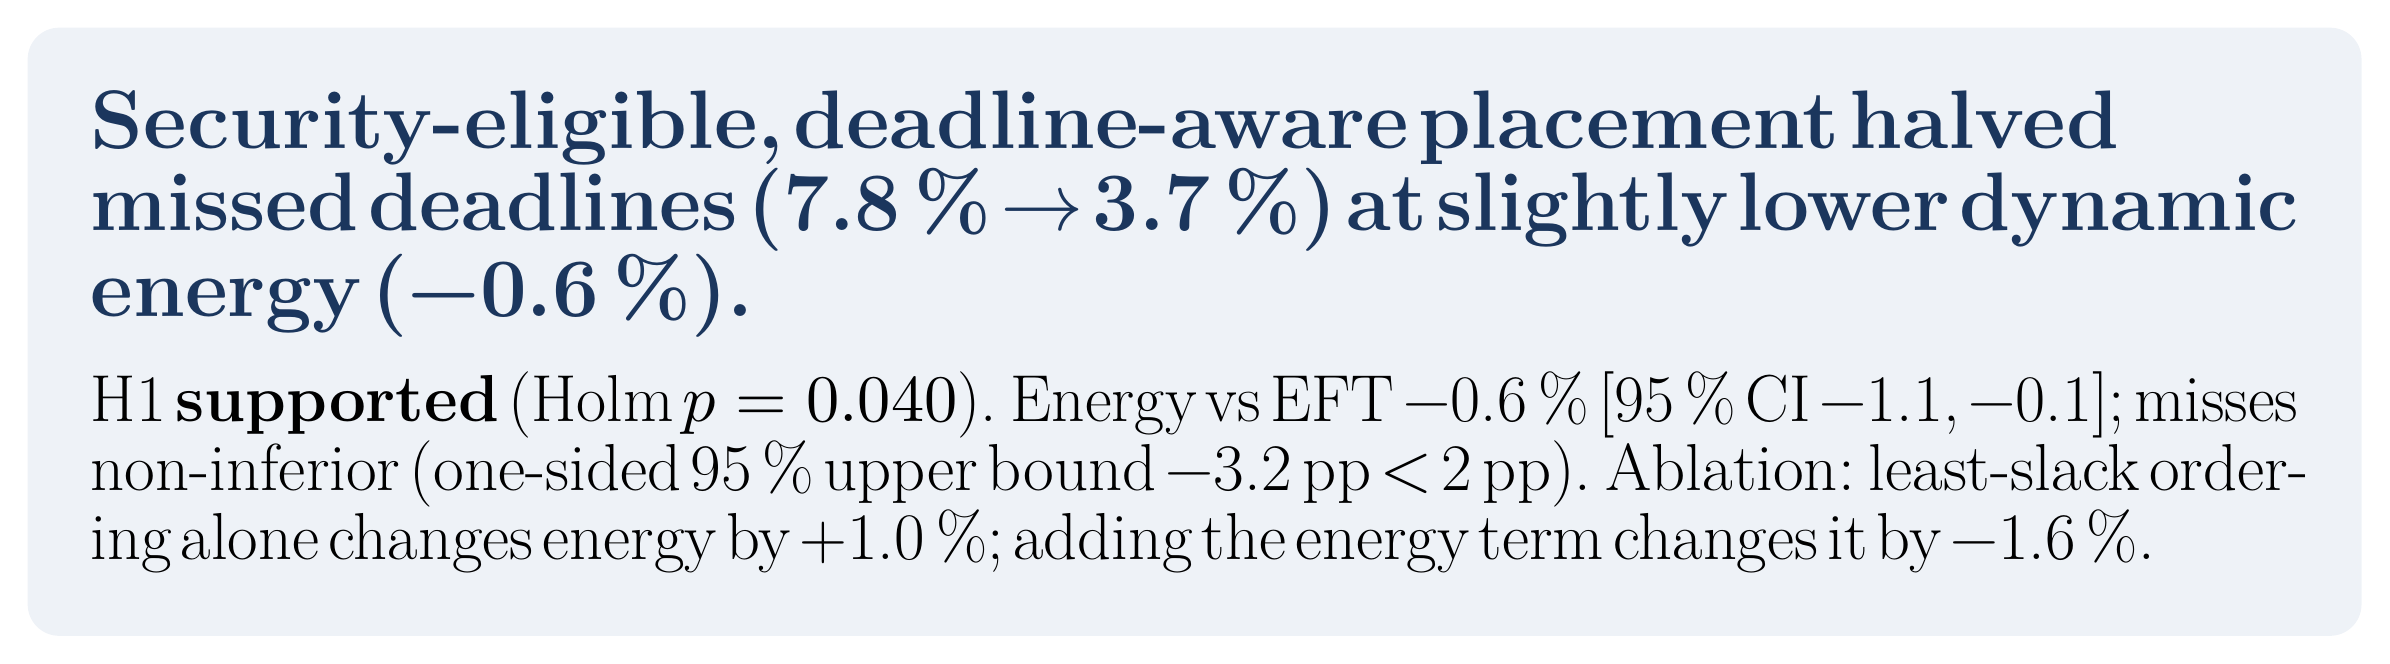
\begin{tikzpicture}
  \node[fill=tint,rounded corners=4mm,inner sep=8mm,text width=\colB-16mm,align=left] {%
    {\fontsize{30}{37}\selectfont\bfseries\color{navy}Security-eligible, deadline-aware placement halved missed deadlines (\HOneMissEft\,\% $\rightarrow$ \HOneMissSeas\,\%) at slightly lower dynamic energy (\HOneEnergyRel\,\%).}\\[4mm]
    {\capsize H1 \textbf{\HOneVerdict} (Holm $p=\HOnePHolm$). Energy vs EFT \HOneEnergyRel\,\% [95\,\% CI \HOneEnergyLo, \HOneEnergyHi]; misses non-inferior (one-sided 95\,\% upper bound \HOneNIUpper\,pp $<$ \HOneNIMargin\,pp). Ablation: least-slack ordering alone changes energy by +\AblSlackVsEft\,\%; adding the energy term changes it by \AblSeasVsSlack\,\%.}};
\end{tikzpicture}
\figfile{figB_S1_energy_miss}
\caption{Modelled dynamic energy and deadline-miss rate per policy; mean and 95\,\% bootstrap CI over 30 paired seeds. FIFO-FF bar truncated (value printed).}
\figfile{figB2_S1_rel_energy}
\caption{Same runs, paired per seed: dynamic energy relative to EFT. Dots = seeds, diamonds = mean with 95\,\% CI.}

\section{Security constraints shrink the gain (H2 refuted)}
\begin{minipage}[c]{180mm}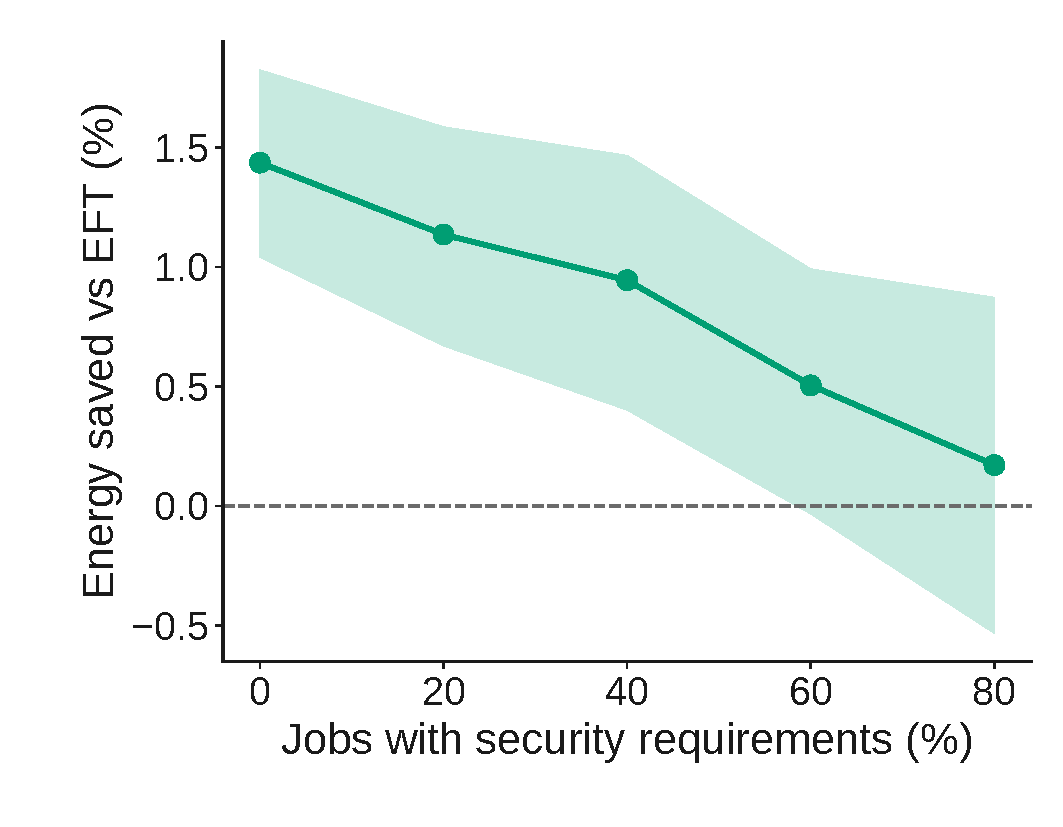
\includegraphics{figS4_gain_vs_security.pdf}\end{minipage}\hfill
\begin{minipage}[c]{\dimexpr\colB-186mm}\capsize\raggedright
H2 \textbf{\HTwoVerdict}: the gain fell from \HTwoGainZero\,\% to \HTwoGainMax\,\% as secure jobs rose to 80\,\% (slope \HTwoSlope\,pp per 100\,\% secure jobs, CI [\HTwoSlopeLo, \HTwoSlopeHi]). Constraints remove choices before energy can be optimised.
\end{minipage}
\end{minipage}\end{lrbox}%
% ===================== COLUMN 3 =====================
\begin{lrbox}{\boxC}\begin{minipage}[t]{\colA}\vspace{0pt}
\firstsection{What the numbers mean}
\begin{itemize}
  \item \textbf{Placement leverage is small here.} Even deadline-blind energy-greedy changes energy by only \GreedyEnergyRel\,\% vs \seasname{}, while missing \HFourDiff\,pp more deadlines (H4: deadlines \HFourVerdict).
  \item \textbf{Idle power dominates.} Dynamic energy is \DynShare\,\% of the always-on total; vs EFT, total energy changes by \TotCommonRel\,\%.
  \item \textbf{Under ideal power-gating} the saving vanishes (\TotGatedRel\,\%, CI [\TotGatedLo, \TotGatedHi]): \seasname{} keeps CPUs busy longer.
  \item \seasname{} completes \WorkRel\,\% more work, so its energy per unit of completed work changes by \PerWorkRel\,\% [\PerWorkLo, \PerWorkHi] {\color{muted}(secondary, not preregistered)}.
  \item Robust to estimation error (H3 \HThreeVerdict, Holm $p=\HThreePHolm$). The energy weight acts as a switch: $\alpha\ge0.25$ gives identical schedules.
\end{itemize}
\vspace{3mm}
{\bfseries\color{navy}Next question:} placement must be co-optimised with power states and measured, not modelled, energy.

\section{Research roadmap}
\begin{center}
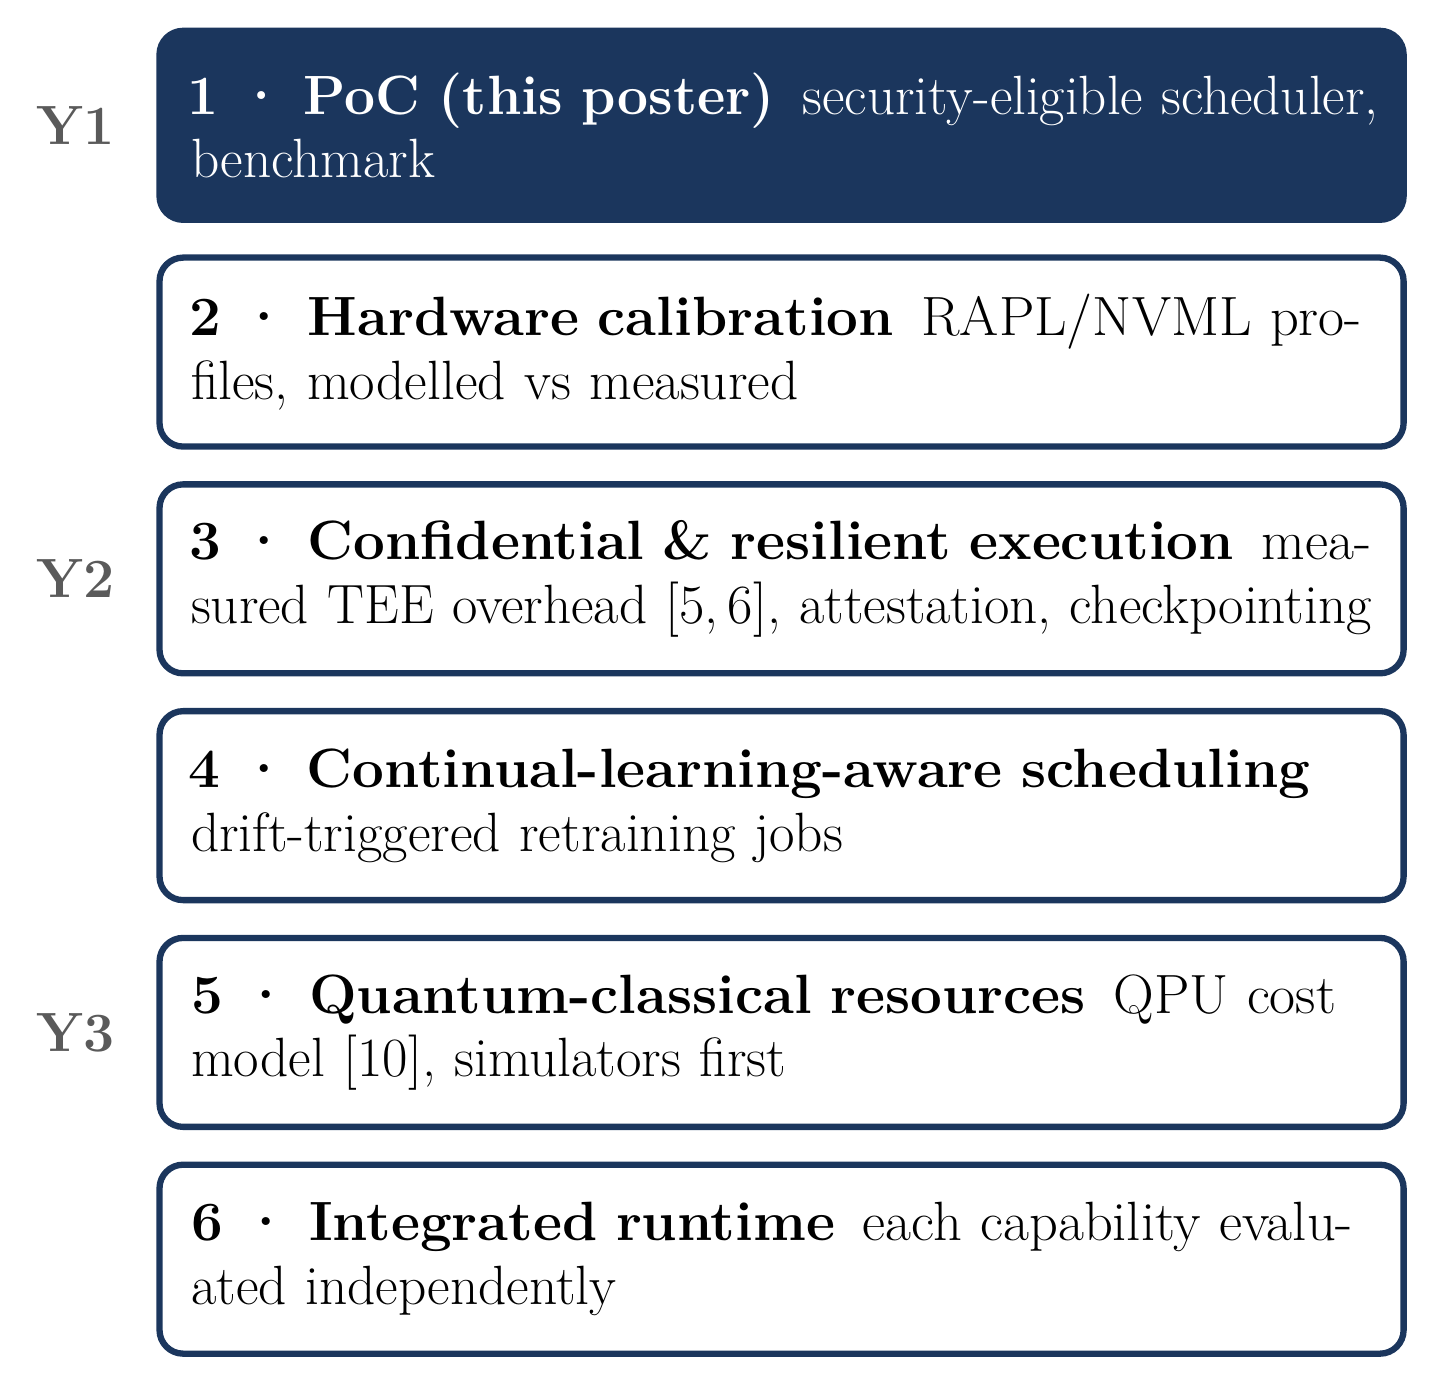
\begin{tikzpicture}[font=\fontsize{20}{23}\selectfont,
   st/.style={draw=navy,line width=0.8mm,rounded corners=3mm,minimum height=24mm,text width=150mm,align=left,inner sep=4mm},
   done/.style={st,fill=navy,text=white},
   todo/.style={st,fill=white},
   yr/.style={font=\fontsize{20}{23}\selectfont\bfseries,text=muted,anchor=east}]
  \node[done] (s1) {\textbf{1 · PoC (this poster)}\, security-eligible scheduler, benchmark};
  \node[todo,below=4mm of s1] (s2) {\textbf{2 · Hardware calibration}\, RAPL/NVML profiles, modelled vs measured};
  \node[todo,below=4mm of s2] (s3) {\textbf{3 · Confidential \& resilient execution}\, measured TEE overhead [5,\,6], attestation, checkpointing};
  \node[todo,below=4mm of s3] (s4) {\textbf{4 · Continual-learning-aware scheduling}\, drift-triggered retraining jobs};
  \node[todo,below=4mm of s4] (s5) {\textbf{5 · Quantum-classical resources}\, QPU cost model [10], simulators first};
  \node[todo,below=4mm of s5] (s6) {\textbf{6 · Integrated runtime}\, each capability evaluated independently};
  \node[yr] at ([xshift=-4mm]s1.west) {Y1};
  \node[yr] at ([xshift=-4mm]s3.west) {Y2};
  \node[yr] at ([xshift=-4mm]s5.west) {Y3};
\end{tikzpicture}
\end{center}

\section{Open research work}
{\capsize
\begin{itemize}
  \item \textbf{Scheduling \& optimisation} — exact bounds, power-state-aware policies.
  \item \textbf{Energy profiling} — calibrate CPU/GPU power; validate the model.
  \item \textbf{Secure execution} — measure TEE overhead per job type.
  \item \textbf{Continual learning} — retraining streams and staleness metrics.
  \item \textbf{Quantum-classical} — a QPU node class in the same model.
\end{itemize}
\vspace{3mm}
Contributions start from a labelled first issue in the repository; reproducing every figure takes one command.\par}
\vspace{4mm}
{\bfseries\color{navy}Contact:} costin.deonise@upb.ro

\section{References}
{\refsize
[1]~Wang et al., DVFS-enabled heterogeneous clusters, \emph{IEEE TPDS} 33(12), 2022.
[2]~Chau et al., DVFS for CPU-GPU systems, \emph{ACM e-Energy}, 2017.
[3]~Topcuoglu et al., HEFT, \emph{IEEE TPDS} 13(3), 2002.
[4]~You et al., Zeus, \emph{USENIX NSDI}, 2023.
[5]~Mo et al., ML with confidential computing (SoK), \emph{ACM CSUR} 56(11), 2024.
[6]~Zhu et al., Confidential computing on H100, arXiv:2409.03992, 2024.
[7]~Luccioni et al., Power hungry processing, \emph{ACM FAccT}, 2024.
[8]~Schwartz et al., Green AI, \emph{CACM} 63(12), 2020.
[9]~Aczel et al., Environmental cost of AI's energy use, UNU-INWEH, 2026.
[10]~Beck et al., QC in HPC ecosystems, \emph{FGCS} 161, 2024.\par}

\vspace{8mm}
{\refsize\color{muted}\textbf{Acknowledgements.} Supervision: Prof.\ Dr.\ Eng.\ Florin Pop. PRECIS Research Centre, National University of Science and Technology POLITEHNICA Bucharest. State-funded doctoral position; no project grant is associated with this work.\par}
\end{minipage}\end{lrbox}%
\typeout{COLHEIGHT A=\the\dimexpr\ht\boxA+\dp\boxA\relax\space B=\the\dimexpr\ht\boxB+\dp\boxB\relax\space C=\the\dimexpr\ht\boxC+\dp\boxC\relax\space AVAIL=\the\dimexpr 1189mm-\toppos-26mm\relax}%
\begin{tikzpicture}[remember picture,overlay]
  \node[anchor=north west,inner sep=0] at ([xshift=30mm,yshift=-\toppos]current page.north west) {\usebox{\boxA}};
  \node[anchor=north west,inner sep=0] at ([xshift=30mm+\colA+\gut,yshift=-\toppos]current page.north west) {\usebox{\boxB}};
  \node[anchor=north west,inner sep=0] at ([xshift=30mm+\colA+\colB+2\gut,yshift=-\toppos]current page.north west) {\usebox{\boxC}};
\end{tikzpicture}
\end{document}
